\documentclass[a4paper,fleqn,usenatbib]{mnras}
\usepackage{newtxtext,newtxmath}
%\usepackage{mathptmx}
%\usepackage{txfonts}
\usepackage[T1]{fontenc}
\usepackage{ae,aecompl}
\usepackage{graphicx}	% Including figure files
\usepackage{amsmath}	% Advanced maths commands
\usepackage{amssymb}	% Extra maths symbols
\usepackage{color,ulem}
\newcommand{\St}{\mathrm{St}}         % Stokes number
\pdfminorversion=5

%%%%%%%%%%%%%%%%%%% TITLE PAGE %%%%%%%%%%%%%%%%%%%

\title[Self-induced dust traps]{Erratum: Self-induced dust traps: overcoming planet formation barriers}

\author[J.-F. Gonzalez et al.]{
J.-F. Gonzalez,$^{1}$\thanks{E-mail: jean-francois.gonzalez@ens-lyon.fr}
G. Laibe,$^{1,2}$\thanks{E-mail: guillaume.laibe@ens-lyon.fr}
and S. T. Maddison,$^{3}$
\\
$^{1}$Univ Lyon, Univ Lyon1, Ens de Lyon, CNRS, Centre de Recherche Astrophysique de Lyon UMR5574, F-69230, Saint-Genis-Laval, France\\
$^{2}$School of Physics and Astronomy, University of Saint Andrews,
North Haugh, St Andrews, Fife KY16 9SS, UK\\
$^{3}$Centre for Astrophysics and Supercomputing, Swinburne University of Technology, PO Box 218, Hawthorn, VIC 3122, Australia
}

\date{Accepted 2017 August 3. Received 2017 July 10; in original form 2017 July 10.}

\pubyear{2017}

\begin{document}
\label{firstpage}
\pagerange{\pageref{firstpage}--\pageref{lastpage}}
\maketitle

%\begin{abstract}
%\end{abstract}

\begin{keywords}
errata, addenda -- hydrodynamics -- methods: numerical -- protoplanetary discs
\end{keywords}

%%%%%%%%%%%%%%%%%%%%%%%%%%%%%%%%%%%%%%%%%%%%%%%%%%

%%%%%%%%%%%%%%%%% BODY OF PAPER %%%%%%%%%%%%%%%%%%

After publication of the paper `Self-induced dust traps: overcoming planet formation barriers' in MNRAS 467, 1984 (2017), we discovered an inconsequential error in Appendix~C.

Steady-state expressions of the radial velocities for both the gas and dust phases of a dusty disc, taking into account the back-reaction of dust on gas, have been calculated by several authors, for different conditions \citep[e.g.][]{Nakagawa1986,Kretke2009,Dipierro2017,Kanagawa2017}. They are usually written as functions of the Stokes number for the gas-dust mixture $\St'$ and the dust-to-gas ratio $\epsilon=\rho_\mathrm{d}/\rho_\mathrm{g}$. In equation~(C1), we gave the steady-state expression of the radial velocity of the viscous gas phase of a dusty disc as a function of the more commonly used Stokes number defined for the dust only, $\St$, related to $\St'$ by $\St'=\St/(1+\epsilon)$ \citep{Price2015}:
%
\begin{equation}
\begin{array}{r@{\ }c@{\ }l}
v_\mathrm{g} 
& = & -f_\mathrm{drag} \, \displaystyle\frac{1}{\Sigma_\mathrm{g} \Omega} \frac{\partial}{\partial r}\left(c_\mathrm{s}^2 \Sigma_\mathrm{g} \right) + f_\mathrm{visc} \, \frac{\displaystyle\frac{\partial}{\partial r}\left( \Sigma_\mathrm{g} \nu r^3 \frac{\partial \Omega}{\partial r} \right)}{r \Sigma_\mathrm{g} \displaystyle \frac{\partial}{\partial r} \left( r^2 \Omega \right)}, \\
& \equiv & v_\mathrm{g,drag} + v_\mathrm{g,visc} ,
\label{eq:vgr}
\end{array}
\end{equation}
%
where
%
\begin{equation}
f_\mathrm{drag} = \frac{\epsilon}{(1 + \epsilon)^2 \St^{-1} + \St} . \label{eq:fdrag}
\end{equation}
%
When replacing $\St'$ by its expression as a function of $\St$, we mistakenly wrote that $f_\mathrm{visc}=1$. The correct expression is
%
\begin{equation}
f_\mathrm{visc} = \frac{(1 + \epsilon)\,\St^{-1} + \St}{(1 + \epsilon)^2 \St^{-1} + \St} . \label{eq:fvisc}
\end{equation}
%
As a consequence, equation~(C10) should now read
%
\begin{equation}
x_\mathrm{br} \equiv \frac{\left| v_\mathrm{g,drag} \right| }{ \left| v_\mathrm{g,visc} \right| } \simeq \frac{1}{\alpha} \frac{f_\mathrm{drag}}{f_\mathrm{visc}},
\label{eq:def_xbr}
\end{equation}
%
and Fig.~C1 should be replaced with the current Fig.~\ref{Fig:x_br}. It shows that both $f_\mathrm{visc}$ and $x_\mathrm{br}$ are little affected for small values of $\epsilon$. For $\epsilon\sim1$, the effect of back-reaction on the gas phase is up to twice as large, strengthening the conclusions of the initial study.

\begin{figure}
\centering
\resizebox{\hsize}{!}{
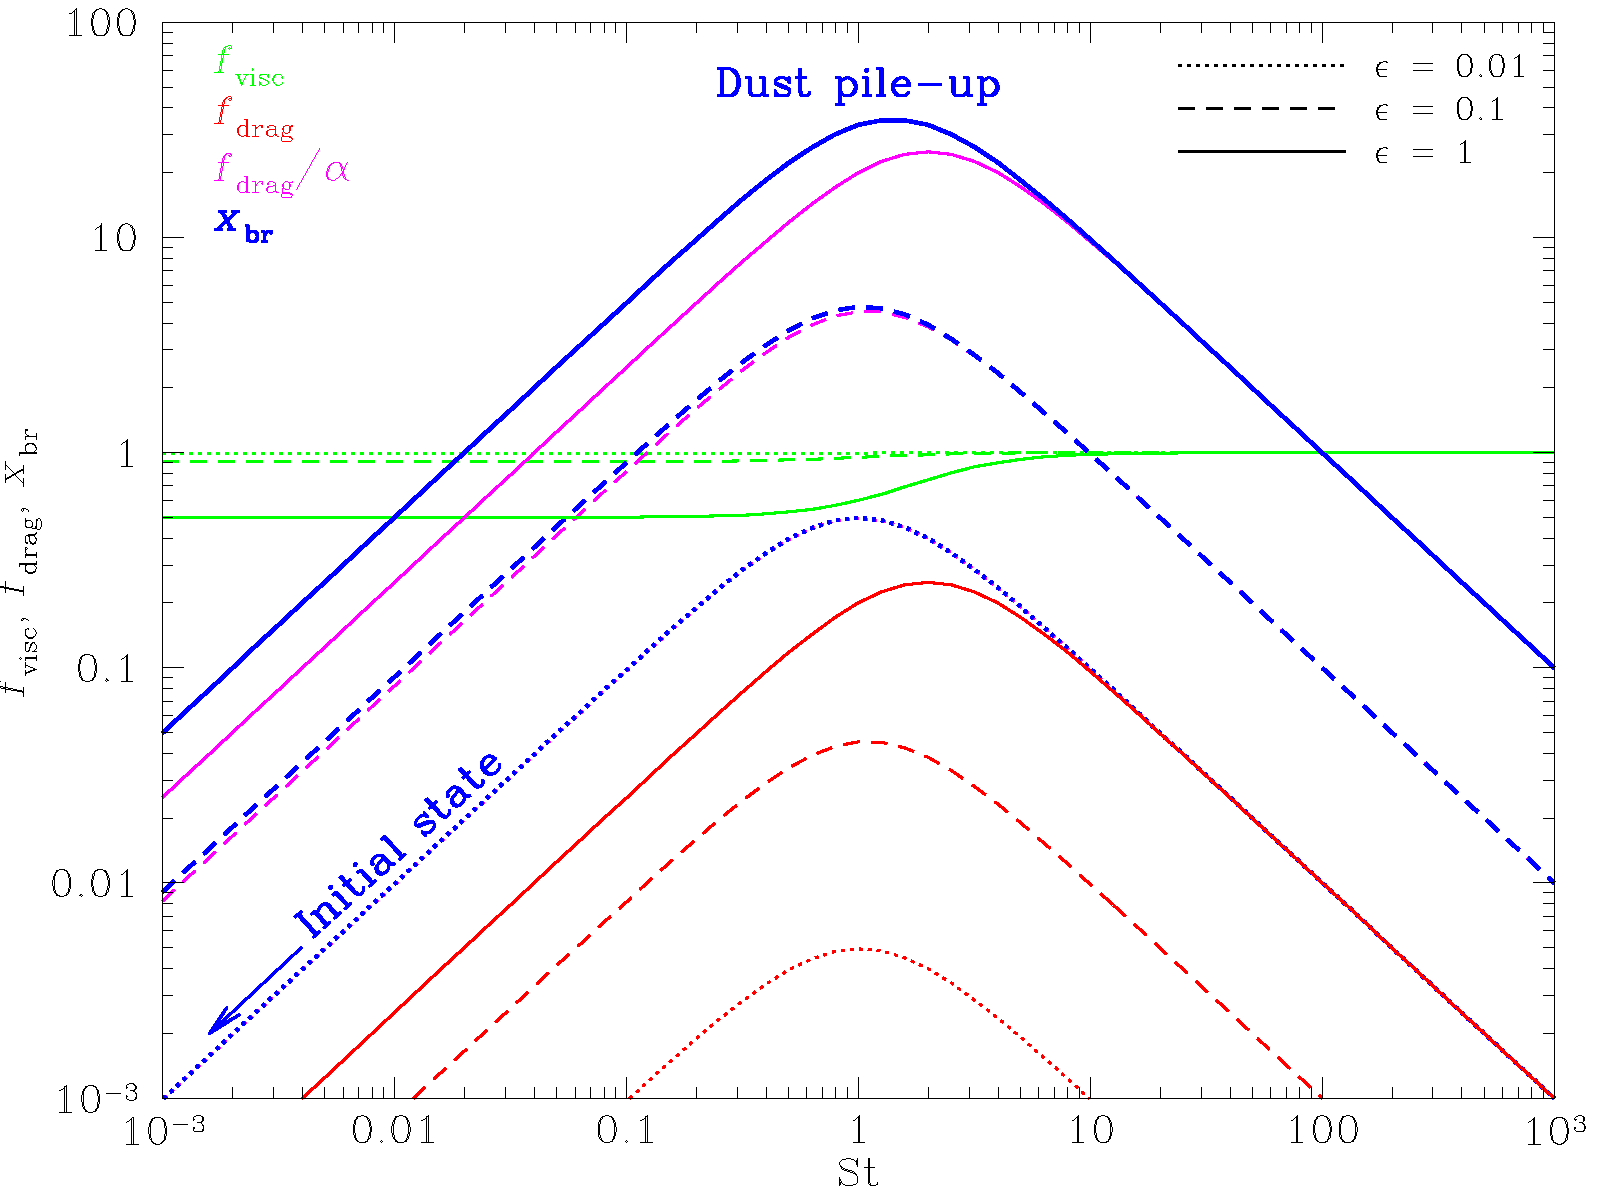
\includegraphics{fig_x_br_erratum.pdf}
}
\caption{Parameter $x_\mathrm{br}$, quantifying the importance of back-reaction on the gas motion, as well as $f_\mathrm{drag}$ and $f_\mathrm{visc}$, as a function of $\St$, for $\epsilon=0.01$, 0.1 and 1, and $\alpha = 10^{-2}$.}
\label{Fig:x_br}
\end{figure}

%\section*{Acknowledgements}
%
%This research was partially supported by the Programme National de Physique Stellaire and the Programme National de Plan\'etologie of CNRS/INSU, France. JFG thanks the LABEX Lyon Institute of Origins (ANR-10-LABX-0066) of the Universit\'e de Lyon for its financial support within the programme `Investissements d'Avenir' (ANR-11-IDEX-0007) of the French government operated by the ANR. GL is grateful for funding from the European Research Council for the FP7 ERC advanced grant project ECOGAL. STM acknowledges partial support from PALSE (Programme Avenir Lyon Saint-Etienne). Simulations were run at the Common Computing Facility (CCF) of LABEX LIO.

%%%%%%%%%%%%%%%%%%%%%%%%%%%%%%%%%%%%%%%%%%%%%%%%%%

%%%%%%%%%%%%%%%%%%%% REFERENCES %%%%%%%%%%%%%%%%%%

\bibliographystyle{mnras}
\bibliography{SelfTraps_Erratum}

%%%%%%%%%%%%%%%%%%%%%%%%%%%%%%%%%%%%%%%%%%%%%%%%%%

% Don't change these lines
\bsp	% typesetting comment
\label{lastpage}
\end{document}

% End of mnras_template.tex